\documentclass{article} \usepackage[margin=1in,headheight=57pt,headsep=0.1in]{geometry}
\usepackage{xcolor}
\usepackage{tikz}
\usepackage{float}
\usepackage{longtable}
\usepackage[framemethod=TikZ]{mdframed}
\usepackage{fancyhdr}
\usepackage[utf8]{inputenc} % Required for inputting international characters
\usepackage[T1]{fontenc} % Output font encoding for international characters
\usepackage{stix} % Use the STIX fonts
\usepackage{hyperref}
\hbadness=99999

% ------------- %
% HEADER/FOOTER %
% ------------- %
\setlength\parindent{0pt}
\setlength\headheight{30pt}
\headsep=0.25in
\lhead{\textbf{Major Project Portfolio: Part 3}}
\rhead{\textbf{12SDD}}


% -------- %
% DOCUMENT %
% -------- %
\begin{document}

% ---------- %
% TITLE PAGE %
% ---------- %
\begin{titlepage} % Suppresses displaying the page number on the title page and the subsequent page counts as page 1

	\raggedleft % Right align the title page

	\rule{1pt}{\textheight} % Vertical line
	\hspace{0.05\textwidth} % Whitespace between the vertical line and title page text
	\parbox[b]{0.75\textwidth}{ % Paragraph box for holding the title page text, adjust the width to move the title page left or right on the page

		{\Huge\bfseries HSC SDD \\[0.5\baselineskip] Major Project Portfolio}\\[2\baselineskip] % Title
		{\large\textit{Part 3: Final Major Project Submission}}\\[4\baselineskip] % Subtitle or further description
		{\Large\textsc{james denovan}} % Author name, lower case for consistent small caps

		\vspace{0.5\textheight} % Whitespace between the title block and the publisher

		{\noindent Kinross Wolarai School}\\[\baselineskip] % Publisher and logo
	}

\end{titlepage}
\thispagestyle{empty}
\tableofcontents
\pagebreak
\pagestyle{fancy}
\section{Implementing the Solution}
\subsection{Algorithms and Psuedocode}
\subsubsection{introForm}
\begin{figure}[H]
	\centering
	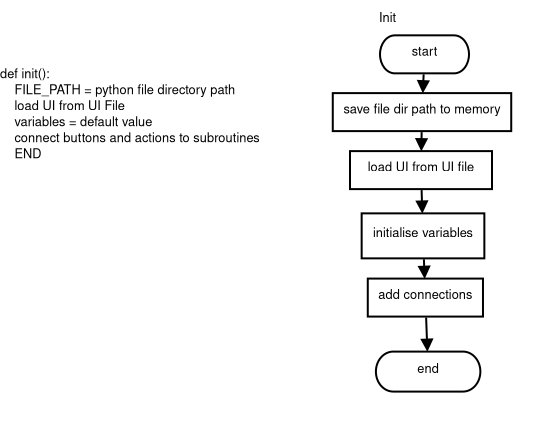
\includegraphics[width=0.8\textwidth]{/home/quiterion/Projects/tbrpggepp/portfolio/Images/introForm1.png}
\end{figure}
\begin{figure}[H]
	\centering
	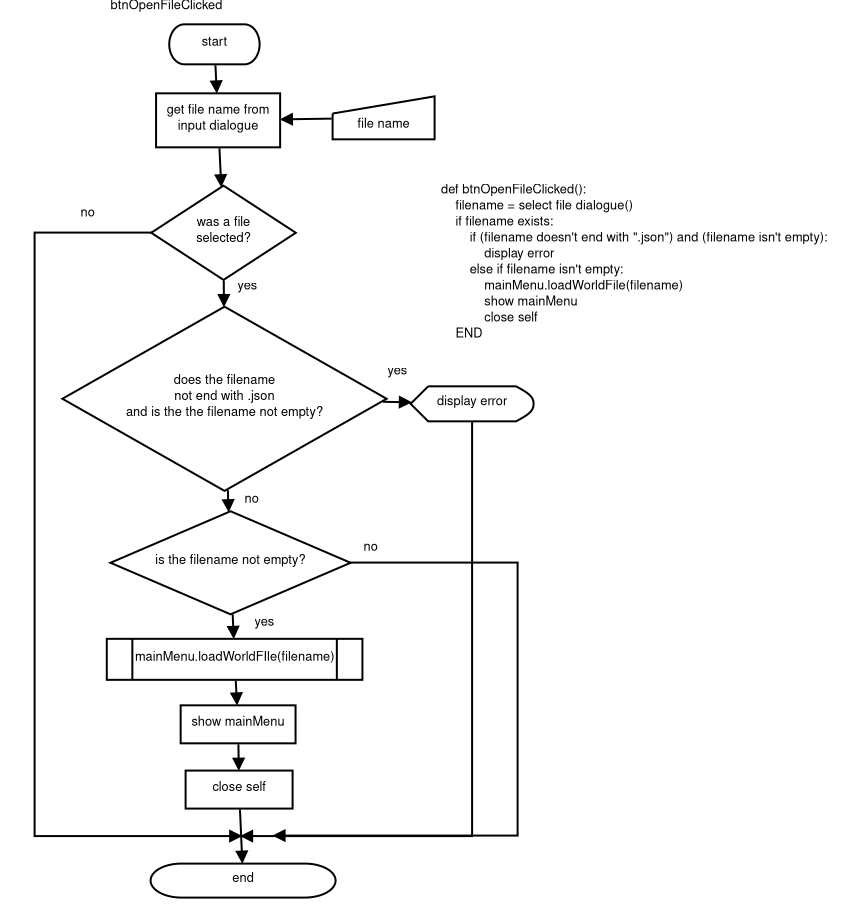
\includegraphics[width=0.8\textwidth]{/home/quiterion/Projects/tbrpggepp/portfolio/Images/introForm2.png}
\end{figure}
\begin{figure}[H]
	\centering
	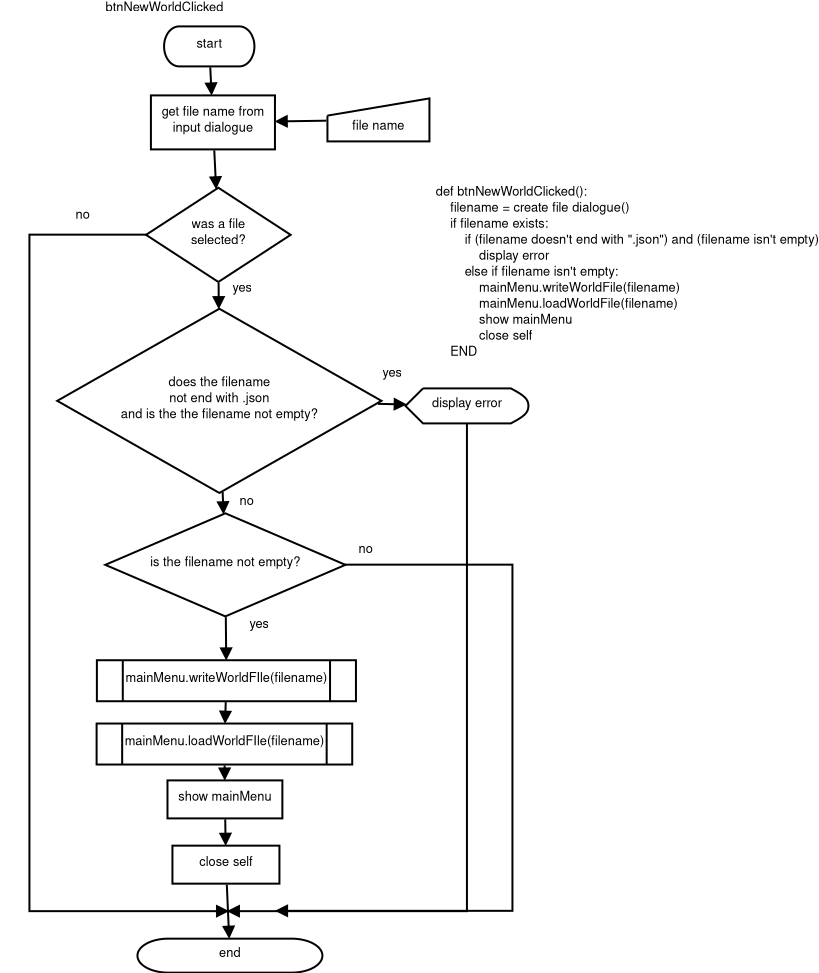
\includegraphics[width=0.8\textwidth]{/home/quiterion/Projects/tbrpggepp/portfolio/Images/introForm3.png}
\end{figure}

\subsubsection{mainMenuForm}
\begin{figure}[H]
	\centering
	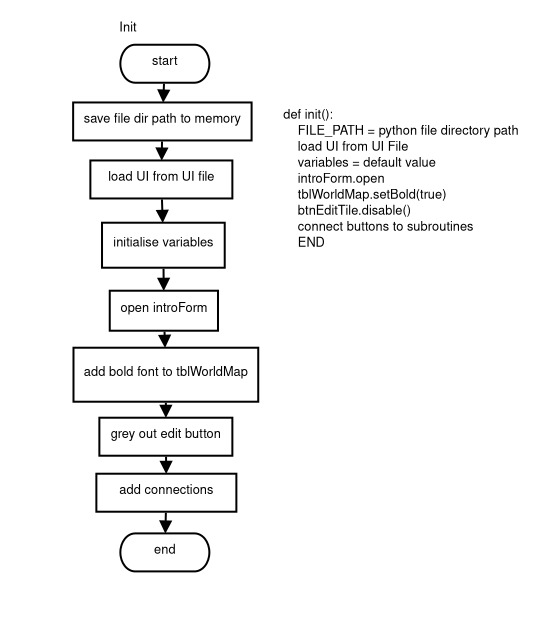
\includegraphics[width=0.8\textwidth]{/home/quiterion/Projects/tbrpggepp/portfolio/Images/mainMenuForm1.png}
\end{figure}
\begin{figure}[H]
	\centering
	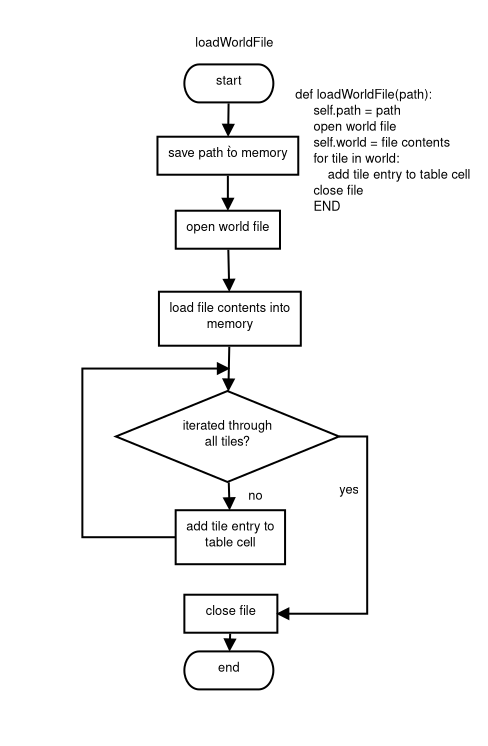
\includegraphics[width=0.8\textwidth]{/home/quiterion/Projects/tbrpggepp/portfolio/Images/mainMenuForm2.png}
\end{figure}
\begin{figure}[H]
	\centering
	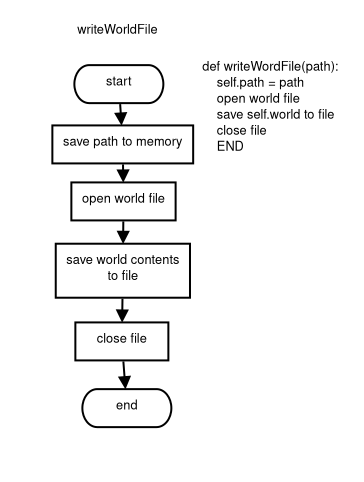
\includegraphics[width=0.8\textwidth]{/home/quiterion/Projects/tbrpggepp/portfolio/Images/mainMenuForm3.png}
\end{figure}
\begin{figure}[H]
	\centering
	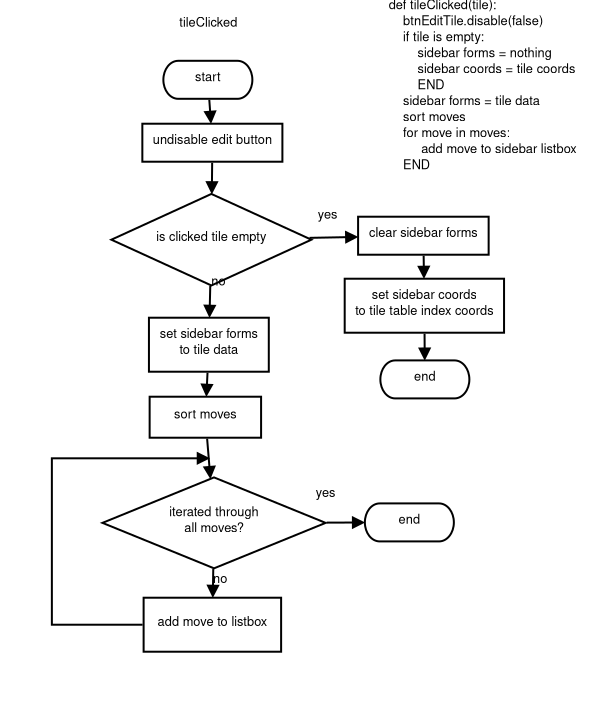
\includegraphics[width=0.8\textwidth]{/home/quiterion/Projects/tbrpggepp/portfolio/Images/mainMenuForm4.png}
\end{figure}
\begin{figure}[H]
	\centering
	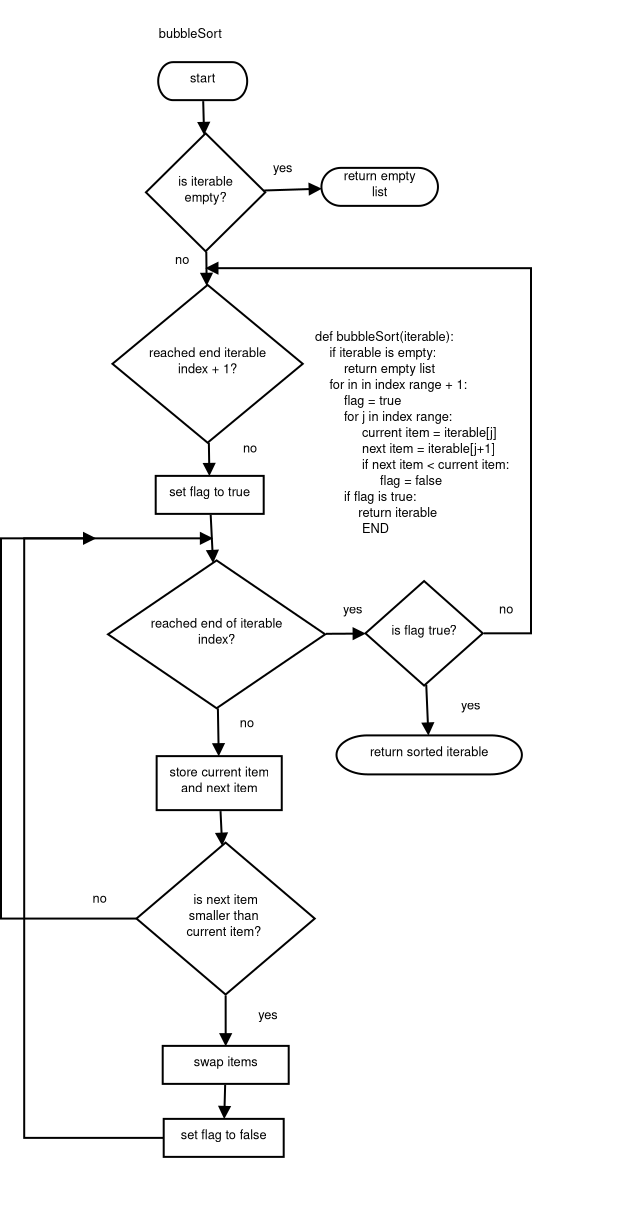
\includegraphics[width=0.8\textwidth]{/home/quiterion/Projects/tbrpggepp/portfolio/Images/mainMenuForm5.png}
\end{figure}
\begin{figure}[H]
	\centering
	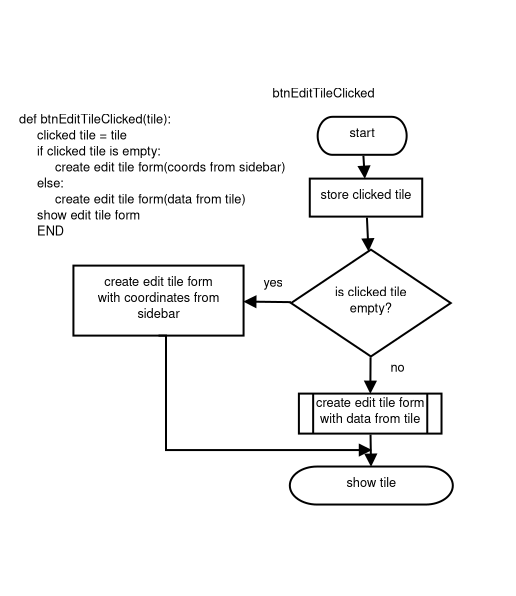
\includegraphics[width=0.8\textwidth]{/home/quiterion/Projects/tbrpggepp/portfolio/Images/mainMenuForm6.png}
\end{figure}
\begin{figure}[H]
	\centering
	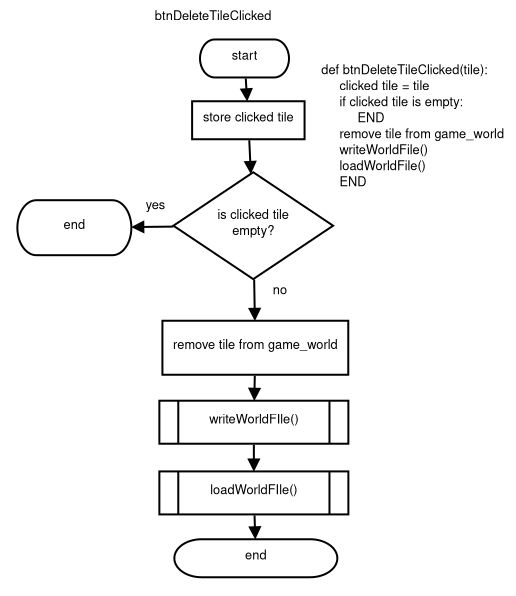
\includegraphics[width=0.8\textwidth]{/home/quiterion/Projects/tbrpggepp/portfolio/Images/mainMenuForm7.png}
\end{figure}
\begin{figure}[H]
	\centering
	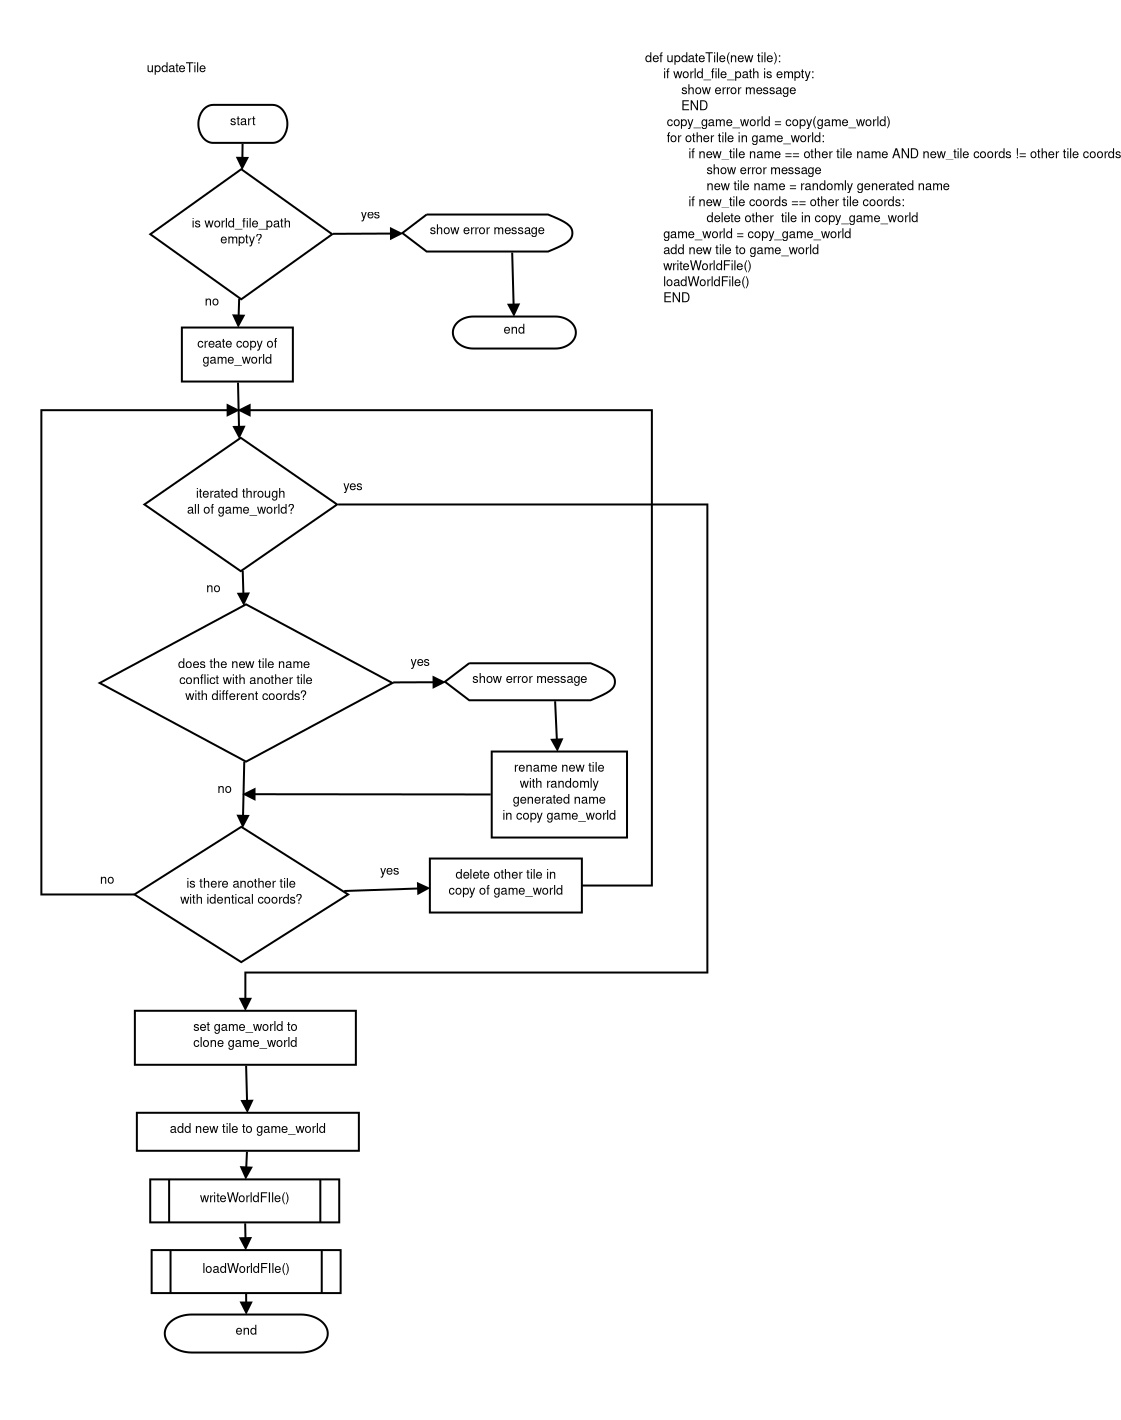
\includegraphics[width=0.8\textwidth]{/home/quiterion/Projects/tbrpggepp/portfolio/Images/mainMenuForm8.png}
\end{figure}
\begin{figure}[H]
	\centering
	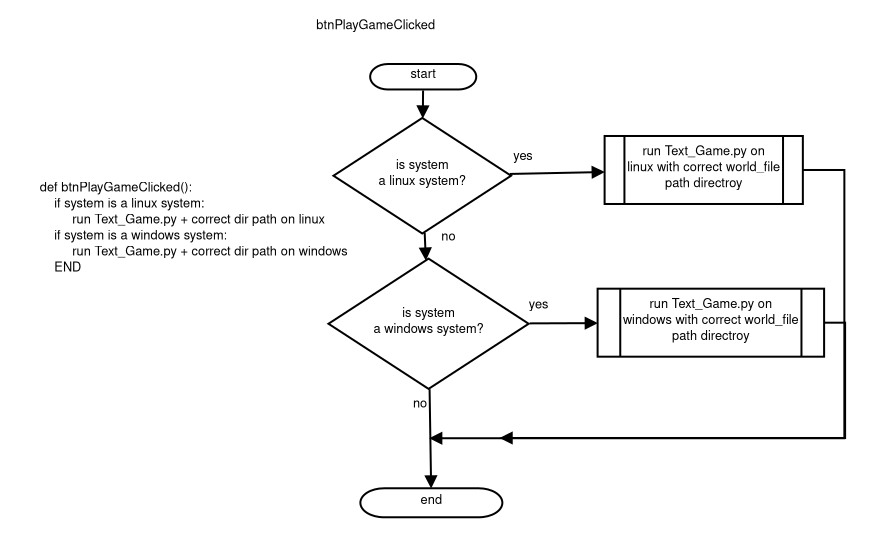
\includegraphics[width=0.8\textwidth]{/home/quiterion/Projects/tbrpggepp/portfolio/Images/mainMenuForm9.png}
\end{figure}
\begin{figure}[H]
	\centering
	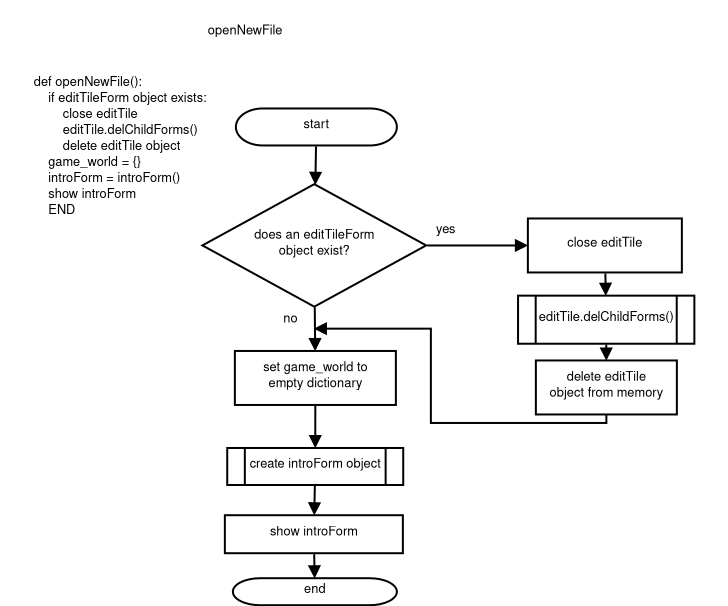
\includegraphics[width=0.8\textwidth]{/home/quiterion/Projects/tbrpggepp/portfolio/Images/mainMenuForm10.png}
\end{figure}

\subsubsection{editTileForm}
\begin{figure}[H]
	\centering
	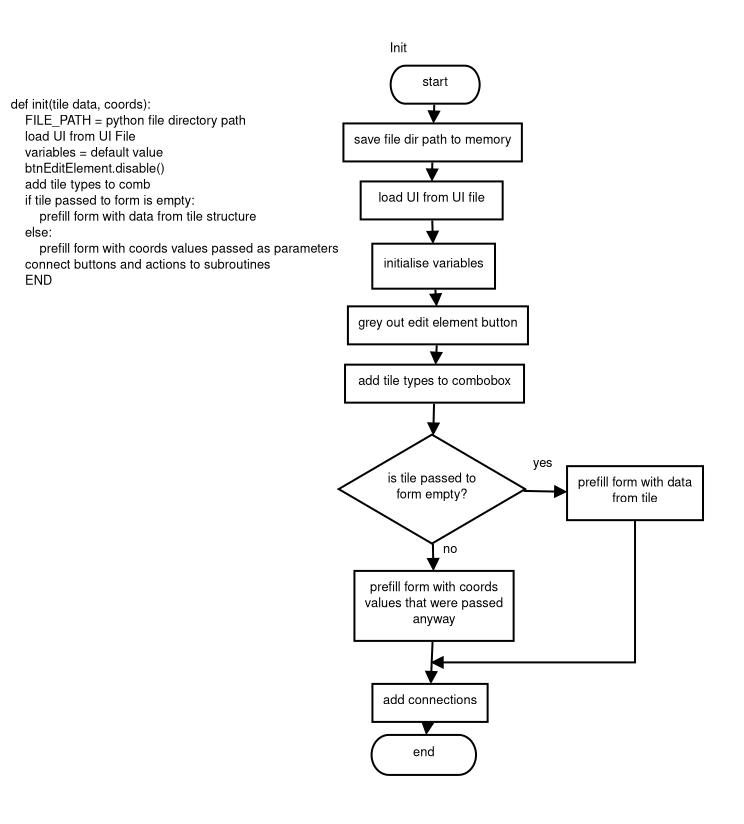
\includegraphics[width=0.8\textwidth]{/home/quiterion/Projects/tbrpggepp/portfolio/Images/editTileForm1.png}
\end{figure}
\begin{figure}[H]
	\centering
	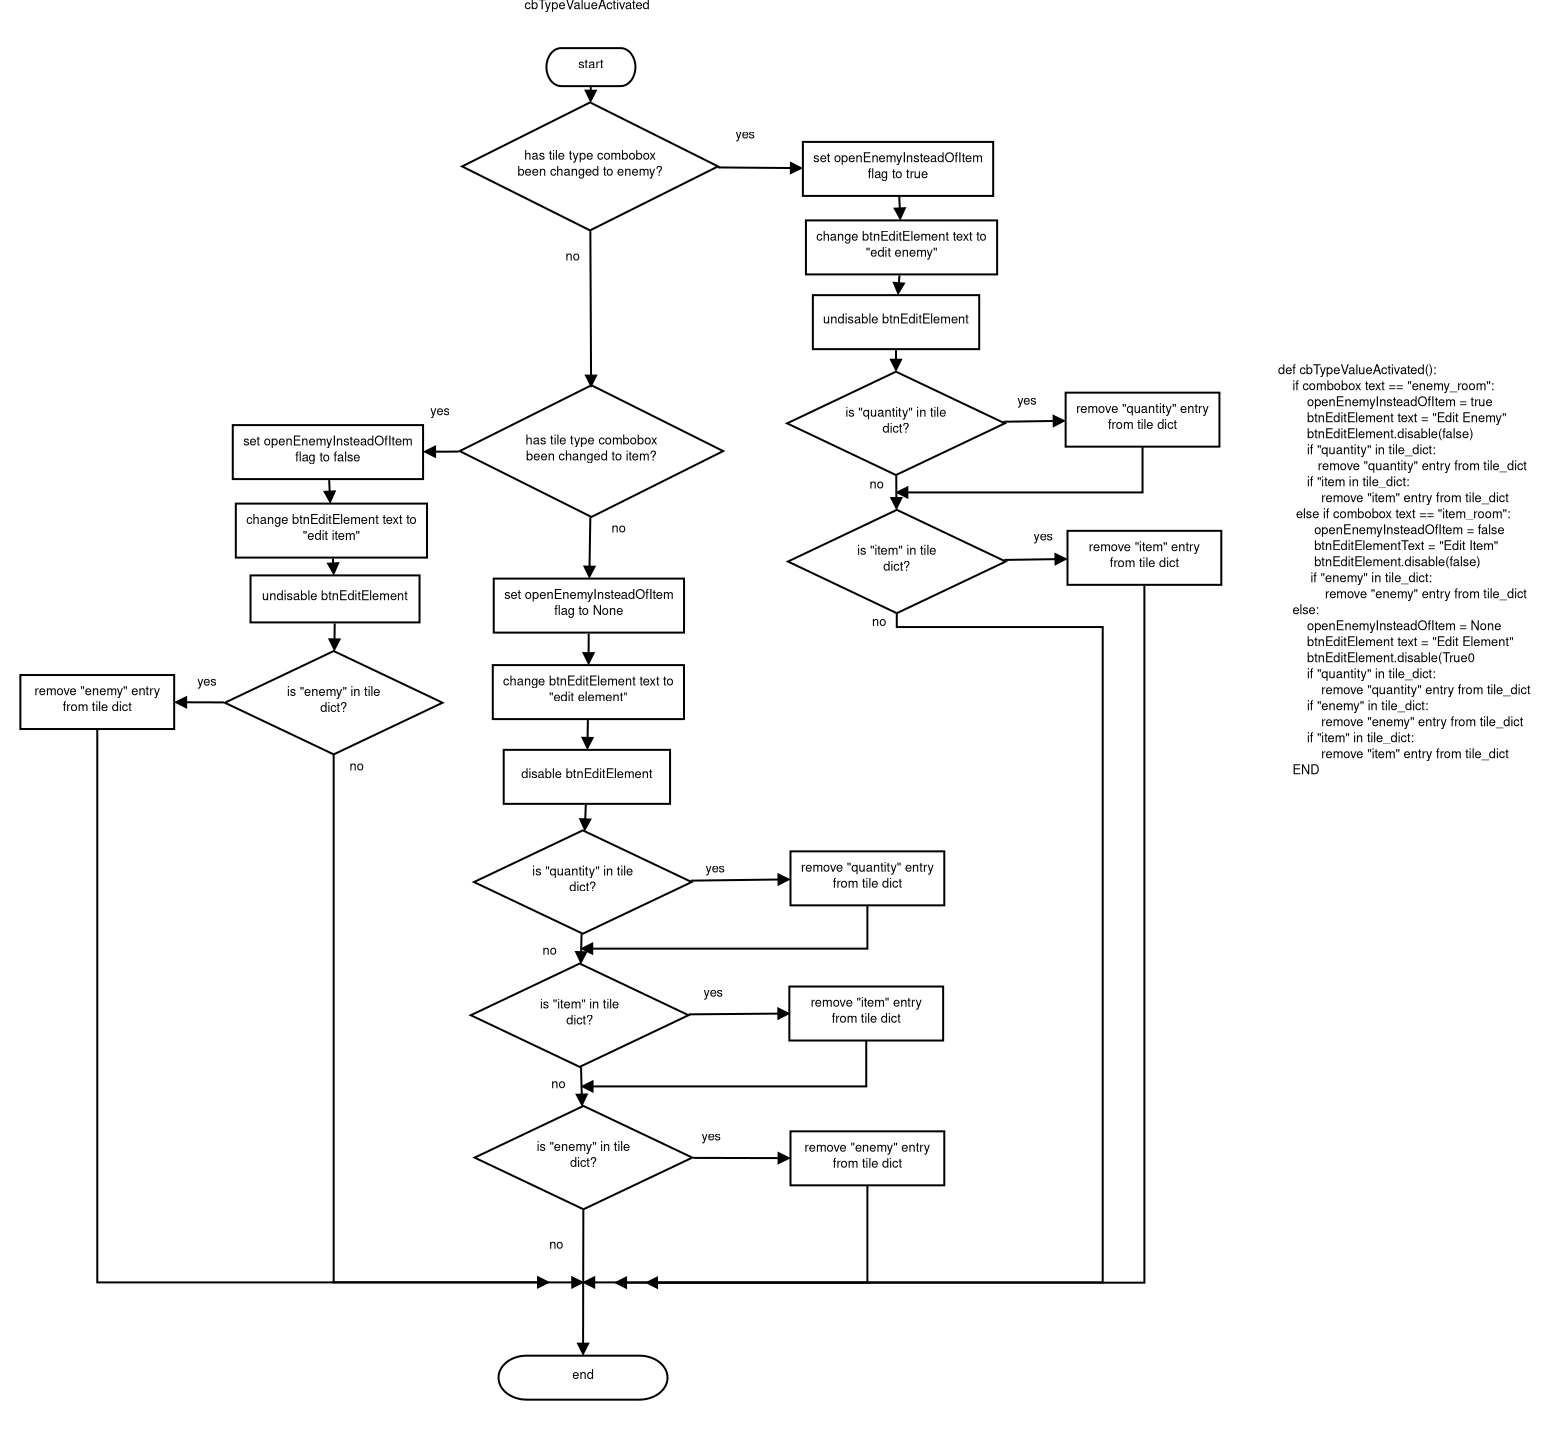
\includegraphics[width=0.8\textwidth]{/home/quiterion/Projects/tbrpggepp/portfolio/Images/editTileForm2.png}
\end{figure}
\begin{figure}[H]
	\centering
	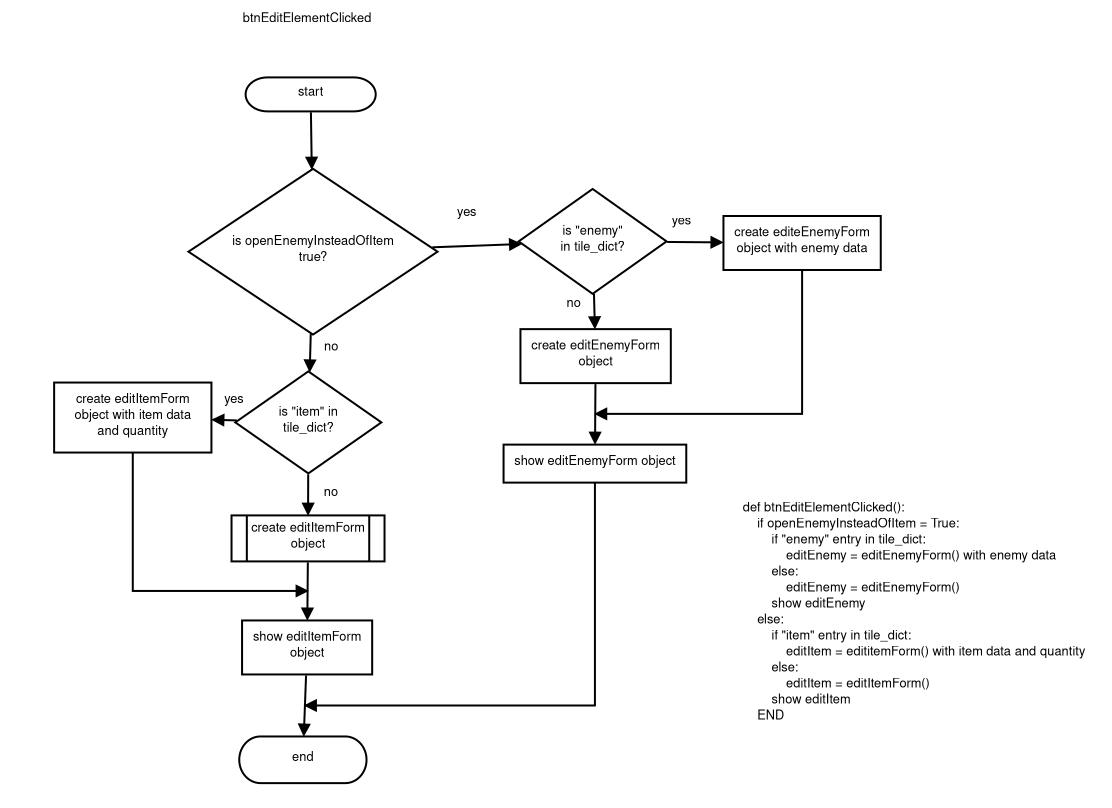
\includegraphics[width=0.8\textwidth]{/home/quiterion/Projects/tbrpggepp/portfolio/Images/editTileForm3.png}
\end{figure}
\begin{figure}[H]
	\centering
	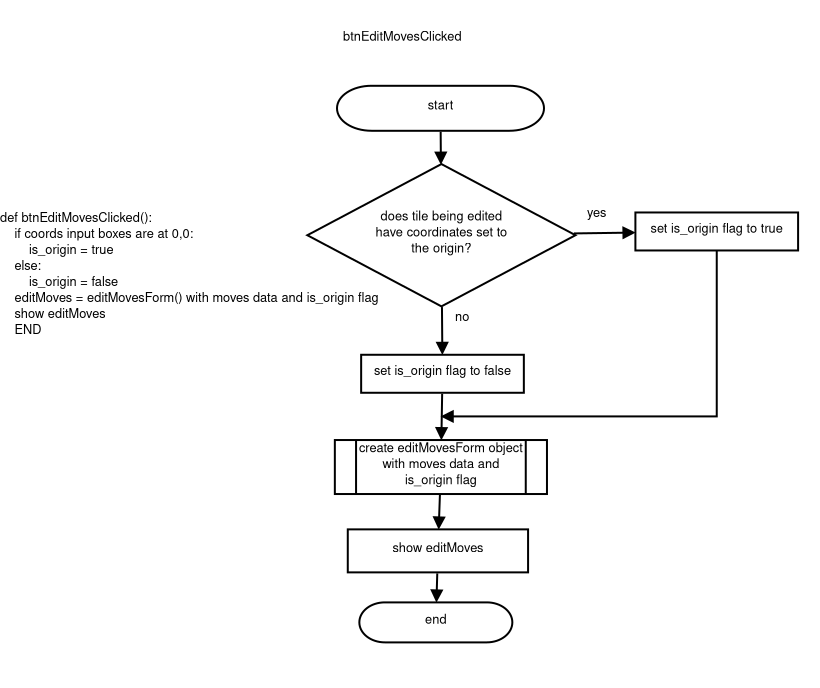
\includegraphics[width=0.8\textwidth]{/home/quiterion/Projects/tbrpggepp/portfolio/Images/editTileForm4.png}
\end{figure}
\begin{figure}[H]
	\centering
	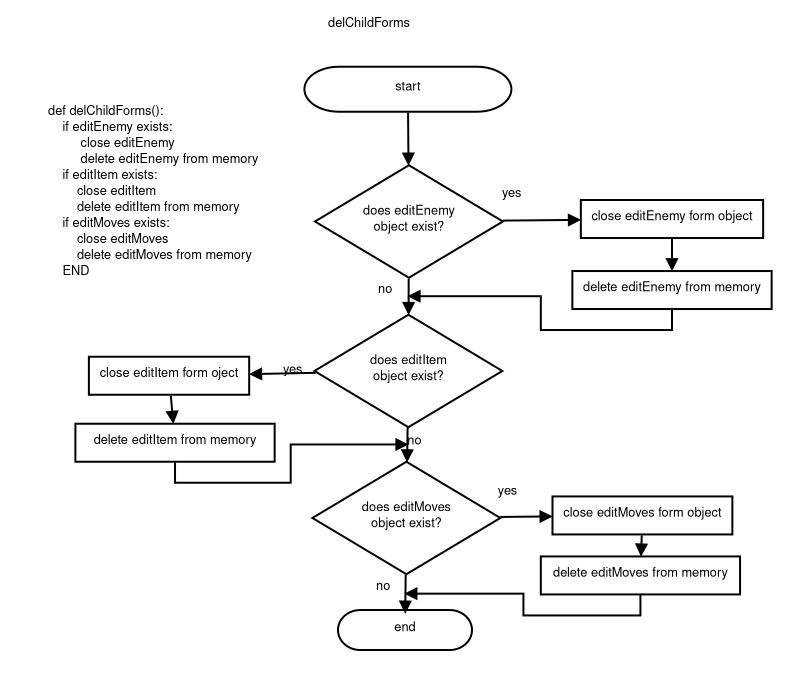
\includegraphics[width=0.8\textwidth]{/home/quiterion/Projects/tbrpggepp/portfolio/Images/editTileForm5.png}
\end{figure}
\begin{figure}[H]
	\centering
	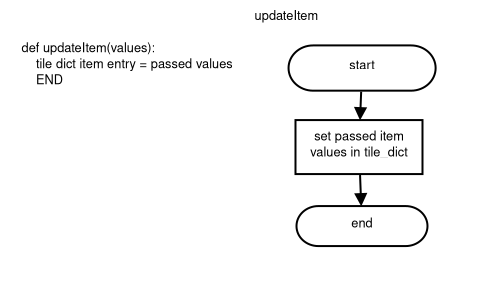
\includegraphics[width=0.8\textwidth]{/home/quiterion/Projects/tbrpggepp/portfolio/Images/editTileForm6.png}
\end{figure}
\begin{figure}[H]
	\centering
	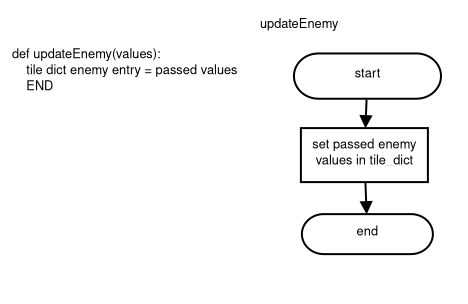
\includegraphics[width=0.8\textwidth]{/home/quiterion/Projects/tbrpggepp/portfolio/Images/editTileForm7.png}
\end{figure}
\begin{figure}[H]
	\centering
	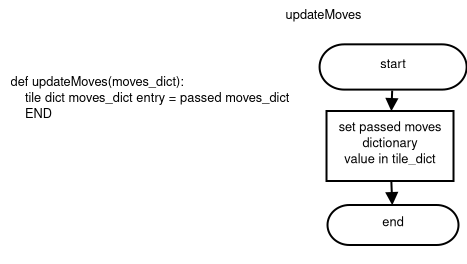
\includegraphics[width=0.8\textwidth]{/home/quiterion/Projects/tbrpggepp/portfolio/Images/editTileForm8.png}
\end{figure}
\begin{figure}[H]
	\centering
	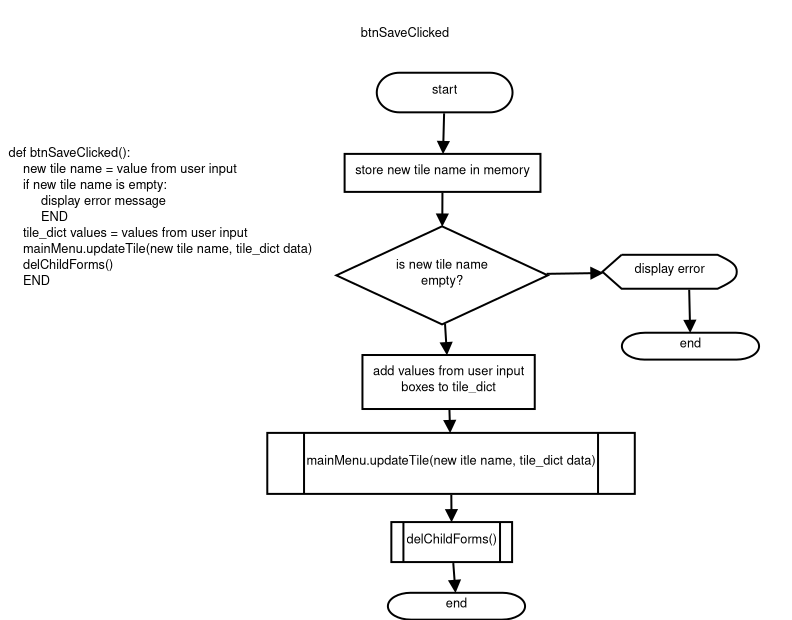
\includegraphics[width=0.8\textwidth]{/home/quiterion/Projects/tbrpggepp/portfolio/Images/editTileForm9.png}
\end{figure}

\subsubsection{editItemForm}
\begin{figure}[H]
	\centering
	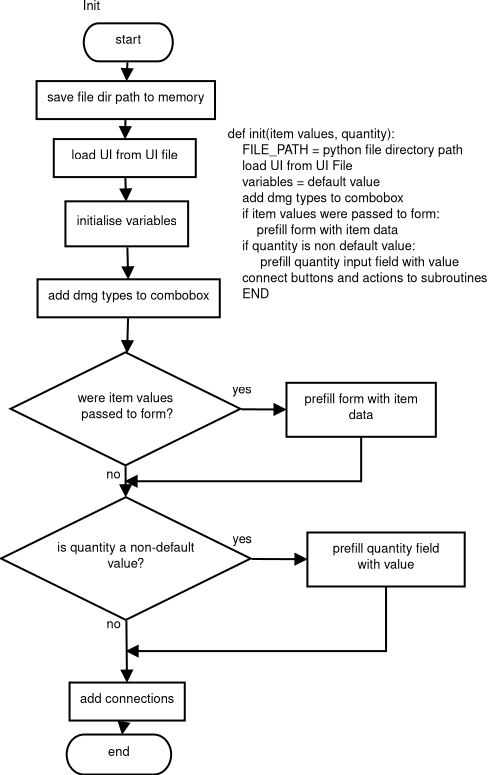
\includegraphics[width=0.8\textwidth]{/home/quiterion/Projects/tbrpggepp/portfolio/Images/editItemForm1.png}
\end{figure}
\begin{figure}[H]
	\centering
	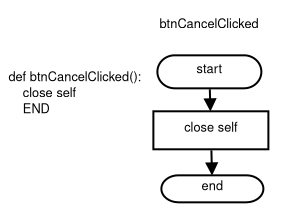
\includegraphics[width=0.8\textwidth]{/home/quiterion/Projects/tbrpggepp/portfolio/Images/editItemForm2.png}
\end{figure}
\begin{figure}[H]
	\centering
	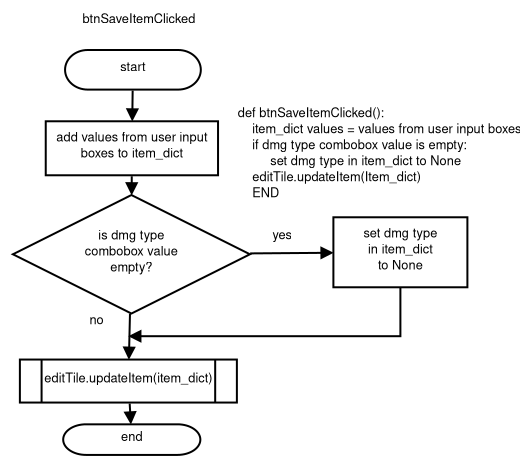
\includegraphics[width=0.8\textwidth]{/home/quiterion/Projects/tbrpggepp/portfolio/Images/editItemForm3.png}
\end{figure}

\subsubsection{editEnemyForm}
\begin{figure}[H]
	\centering
	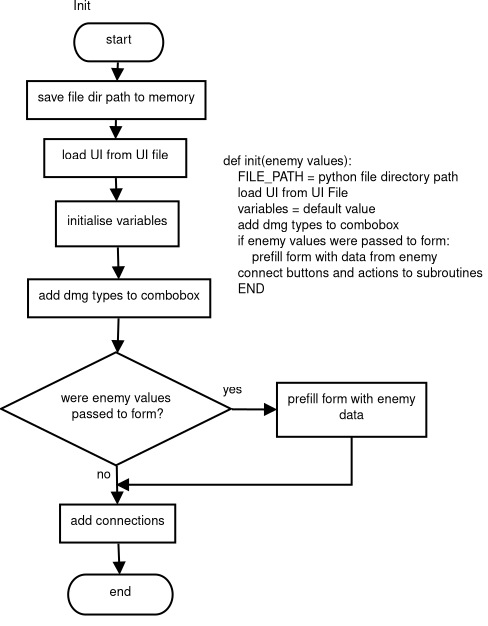
\includegraphics[width=0.8\textwidth]{/home/quiterion/Projects/tbrpggepp/portfolio/Images/editEnemyForm1.png}
\end{figure}
\begin{figure}[H]
	\centering
	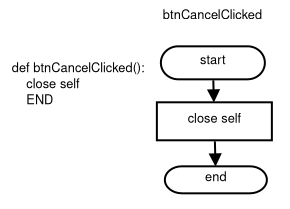
\includegraphics[width=0.8\textwidth]{/home/quiterion/Projects/tbrpggepp/portfolio/Images/editEnemyForm2.png}
\end{figure}
\begin{figure}[H]
	\centering
	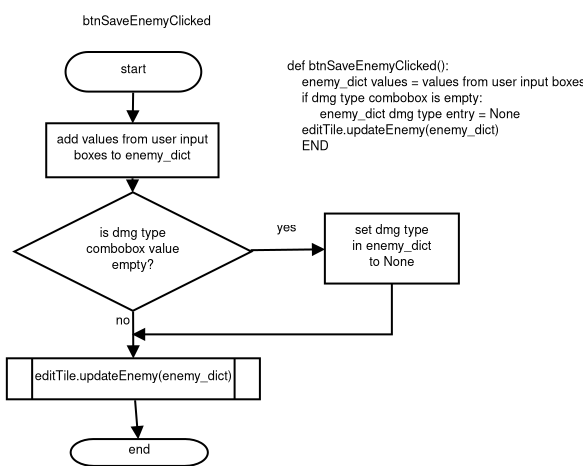
\includegraphics[width=0.8\textwidth]{/home/quiterion/Projects/tbrpggepp/portfolio/Images/editEnemyForm3.png}
\end{figure}

\subsubsection{editMovesForm}
\begin{figure}[H]
	\centering
	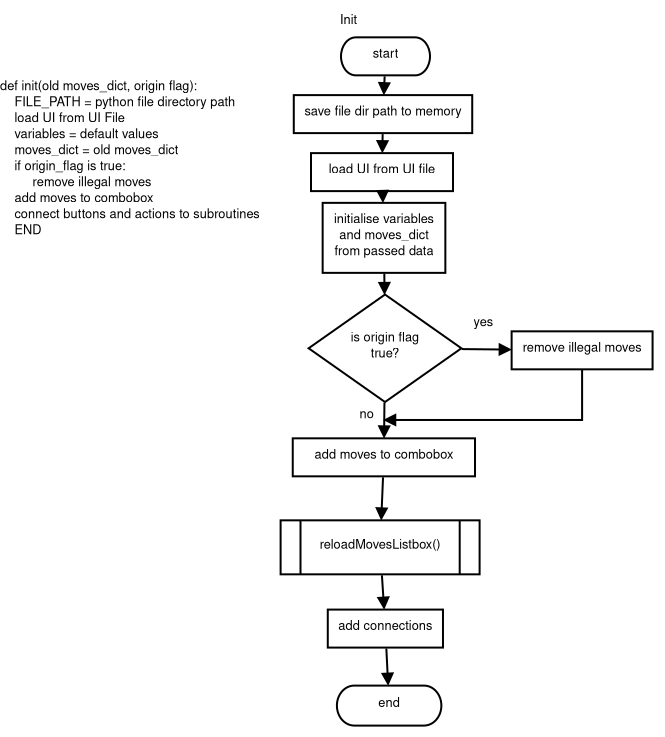
\includegraphics[width=0.8\textwidth]{/home/quiterion/Projects/tbrpggepp/portfolio/Images/editMovesForm1.png}
\end{figure}
\begin{figure}[H]
	\centering
	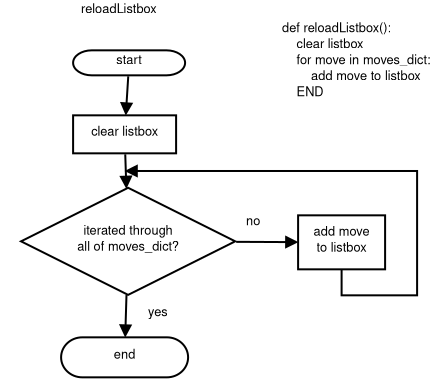
\includegraphics[width=0.8\textwidth]{/home/quiterion/Projects/tbrpggepp/portfolio/Images/editMovesForm2.png}
\end{figure}
\begin{figure}[H]
	\centering
	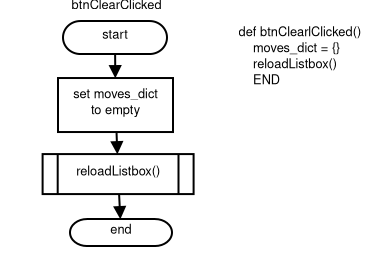
\includegraphics[width=0.8\textwidth]{/home/quiterion/Projects/tbrpggepp/portfolio/Images/editMovesForm3.png}
\end{figure}
\begin{figure}[H]
	\centering
	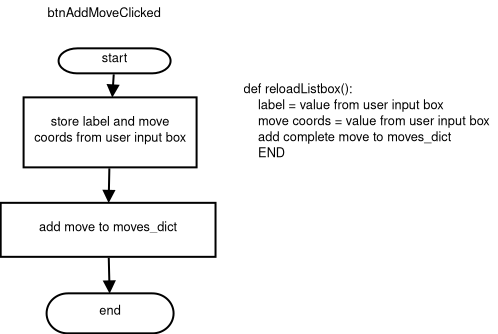
\includegraphics[width=0.8\textwidth]{/home/quiterion/Projects/tbrpggepp/portfolio/Images/editMovesForm4.png}
\end{figure}
\begin{figure}[H]
	\centering
	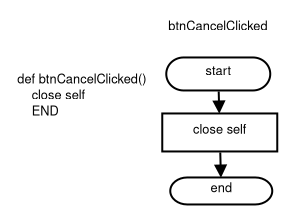
\includegraphics[width=0.8\textwidth]{/home/quiterion/Projects/tbrpggepp/portfolio/Images/editMovesForm5.png}
\end{figure}
\begin{figure}[H]
	\centering
	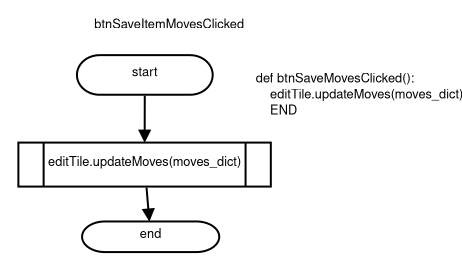
\includegraphics[width=0.8\textwidth]{/home/quiterion/Projects/tbrpggepp/portfolio/Images/editMovesForm6.png}
\end{figure}

\newpage
\subsection{Source Code and User Interface}
Please see: \url{https://github.com/20dj-kws-sdd/tbrpggepp}
\subsection{User Manual}
Please see: \url{https://github.com/20dj-kws-sdd/tbrpggepp/raw/master/manual/manual.pdf}
\newpage
\section{Testing and Maintaining the Solution}
\subsection{Test Plan and Report}
The testing conducted during the development of the program consisted of methodically checking the function of each routine (module-level testing), the methods in which the routines interacted with each other and the program as a whole (program-level testing), and running the program on multiple different operating system environments and checking correct functioning (system-level testing). This was done by enumerating through the permutations of possible input into specific modules and checking if they functioned correctly, and then checking if the modules integrated with each other successfully throughout usage of the program. Near the end of the development phase the program's functioning was checked on a Windows machine as well as the Linux machine the program was developed on, ensuring proper system-level testing. \\

The range of test data used consisted of game-world json files that had been created prior to undergoing this project. The test data ranged from quite small (0 to 6 tiles) to reasonably large (18 full tiles, sufficient for load testing) and was manipulated via operation of the program to enumerate through possible methods of data transformation and ensure continual correct functioning despite the range of possible changes made via program usage. The cross-platform methods for data input, output and transformation were found to be sufficient via system-level testing. \\

The table below contains details of the testing that took place for all modules that involved the input or transformation of data. \\
\begin{center}
	\begin{longtable}[H]{|p{2.9cm}|p{2.9cm}|p{2.9cm}|p{2.9cm}|p{2.9cm}|} \hline
		Item being tested & Test Data being used & Reason for inclusion & Expected Result & Pass/Fail \\ \hline
		btnOpenFileClicked in introForm & non-json file pathname & Test case where user selects invalid file & Error message and no other change & Pass \\ \hline
		btnOpenFileClicked in introForm & empty file pathname & Test case where user cancels file dialog, appearing programmatically as an empty file & No effect & Pass \\ \hline
		btnOpenFileClicked in introForm & valid json file pathname & Ensure ordinary operation of module & mainMenu form opens and loadWorldFile is ran & Pass \\ \hline
		btnNewWorldFileClicked in introForm & non-json file pathname & Test case where user creates invalid file & Error message and no other change & Pass \\ \hline
		btnNewWorldFileClicked in introForm & empty file pathname & Test case where user cancels file dialog, appearing programmatically as an empty file & No effect & Pass \\ \hline
		btnNewWorldFileClicked in introForm & valid json file pathname & Ensure ordinary operation of module & mainMenu form opens and writeWorldFile, then loadWorldFile is ran & Pass \\ \hline
		loadWorldFile in mainMenu & Empty world file (0 tiles) & Test lower bound for data input & Grid appears empty but remains functional & Pass \\ \hline
		loadWorldFile in mainMenu & Small world file (6 tiles) & Test reasonable amount of data input & Tiles load successfully into mainForm & Pass \\ \hline
		loadWorldFile in mainMenu & Large world file (18 tiles) & Load testing for data input & Tiles load successfully into mainForm & Pass \\ \hline
		writeWorldFile in mainMenu & World file paths of varying locations & Test proper functionality of module & Creates file in specified path and dumps game-world contents into it & Pass \\ \hline
		tileClicked in mainMenu & Populated game-world tile indexes & Test proper functionality of module when clicking populated tiles & Relevant sidebar information appears to the right, Edit Tile button ungreys if previously grey & Pass \\ \hline
		tileClicked in mainMenu & Empty game-world tile indexes & Test proper functionality of module when clicking empty tiles & Only coord values are updated in sidebar information, other fields appear blank. Edit Tile button ungreys if previously grey. & Pass \\ \hline
		bubbleSort in mainMenu & arbitrary moves\_dict labels, pulled from populated tile data & Test proper functionality of module & Returns sorted labels, displayed in mainMenu sidebar & Pass \\ \hline
		btnEditTileClicked in mainMenu & Empty tile selected & Test proper functionality of module when attempting to edit empty tiles & Edit Tile form opens with only coordinate values prefilled & Pass \\ \hline
		btnEditTileClicked in mainMenu & Populated tile selected & Test proper functionality of module when attempting to edit populated tiles & Edit Tile form opens with all values prefilled & Pass \\ \hline
		btnDeleteTileClicked in mainMenu & Populated tile selected & Test proper functionality of module when attempting to delete populated tiles & Populated tile in game-world grid is replaced with an empty tile & Pass \\ \hline
		btnDeleteTileClicked in mainMenu & Empty tile selected & Test proper functionality of module when attempting to delete empty tiles & No change & Pass \\ \hline
		updateTile in mainMenu & world file path is empty & Check that an error is caught if the user tries to modify a game-world when in fact no game-world is being edited & Error message displayed and no change applied & Pass \\ \hline
		updateTile in mainMenu & tile data where the new tile name overlaps with a preexisting tile in a different location & Check whether the program overwrites the older conflicting tile against the user's will or not. & Error message displayed, new tile renamed to a randomly generated name, no tiles are overwritten & Pass \\ \hline
		updateTile in mainMenu & tile data where the new tile's coordinates overlap with a preexisting tile in the same location & Check whether the program follows the user's intention of updating a preexisting tile with new data & No error message displayed, older tile is overwritten with new tile data & Pass \\ \hline
		updateTile in mainMenu & ordinary tile data without any conflicting overlap in name or coordinates & Ensure proper functioning of module in ordinary situation & New populated tile created at specified coordinates & Pass \\ \hline
		editTileForm module & tile data from a populated tile & Ensure ordinary operation of module when passed a populated tile & Input fields prefilled with tile data & Pass \\ \hline
		editTileForm module & tile data from an unpopulated tile & Ensure ordinary operation of module when passed an empty tile & Only coorindate Input field prefilled, other fields left blank & Pass \\ \hline
		editTileForm module & item/enemy/moves data & Ensure ordinary operation of module when given data from sub-form & Item/Element/Moves data is saved in local memory & Pass \\ \hline
		editItemForm module & item data from a populated tile & Ensure ordinary operation of module when passed populated item data  & Input fields prefilled with item data & Pass \\ \hline
		editItemForm module & empty item data & Ensure ordinary operation of module when not passed any item data & Input fields left blank & Pass \\ \hline
		editEnemyForm module & enemy data from a populated tile & Ensure ordinary operation of module when passed populated enemy data & Enemy data prefilled in input fields & Pass \\ \hline
		editEnemyForm module & empty enemy data & Ensure ordinary operation of module when not passed any enemy data & Input fields left blank & Pass \\ \hline
		editMovesForm module & moves\_dict data from a populated tile & Ensure ordinary operation of module when passed populated moves\_dict data & Moves data prefilled in input fields and listbox displays moves & Pass \\ \hline
		editMovesForm module & empty moves\_dict data & Ensure ordinary operation of module when not passed any moves\_dict data & Input fields and listbox left blank & Pass \\ \hline
	\end{longtable}
\end{center}

\subsection{Maintenance Overview}
Three possible updates or improvements to the project could be as follows:
\begin{enumerate}
	\item Integrating version control for world-files into program \\
		Additional forms for committing, reverting or branching changes made to the game-world file into a local git repo would greatly improve the user's experience in managing changes made to the game-world throughout the operation of the program. This feature was initially within the program's intended scope, but was left out after realizing it didn't affect the core functionality of the program and the actions performed by the additional forms could still be performed by the user by operating the git program manually.
	\item Adding functionality for deleting specific moves in the editMoves form \\
		In the case of the user making an error in the creation of moves for their tile, a "clear all" button is provided - which inevitably would create annoyance for the user since they may temporarily lose their work on the creation of additional valid moves in the tile. Therefore the feature of removing individual moves from the tile's moves\_dict structure would aid them greatly from a quality-of-life perspective in the usage of the program. This feature was left out of the original scope of the project due to a) apparent difficulty to implement and b) the user may, with some care, take steps to mitagate this data loss such as saving the editMoves form every time a valid move is added and cancelling the form instead of clearing it when a mistake is made.
	\item A search bar for tiles in the mainMenu form \\
		A search bar for tile names in the mainMenu form would assist the user in locating elements of the game-world grid in the case they add to it to the point of vast size. This too would be a useful quality-of-life feature but was left out during implementation (despite being initially within the scope of the project) due to difficulty of implementing and non-essential nature to the functioning of the program.
\end{enumerate}
\section{Documentation and Project Work}
\subsection{Learning Journal}
Please see: \url{https://20dj-kws-sdd.github.io/}
\subsection{Project Work}
\begin{figure}[H]
	\centering
	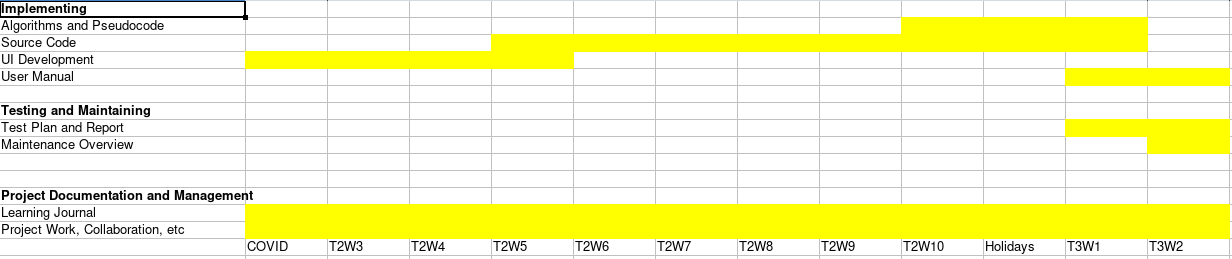
\includegraphics[width=1.0\textwidth]{Images/gantt.png}
\end{figure}
\end{document}
